\section{Dataset}
\label{app:sec:dataset}
% We provide the statistics of the dataset used in our experiments with problems, difficulty statistics and tests in Table \ref{table:platform_comparison}. 

\subsection{Legal compliance and License}
Our benchmark does not comprise and personal identifiable information or offensive content.

Similar to \citep{hendrycks2021measuring}, we scrape only the problem statements, ground-truth solutions, and test cases from competition websites -- \leetcode{}, \atcoder{}, and \codeforces{}. 
Further, we primarily scrape publicly visible portions of websites, avoiding any data collection that might be pay-walled or require login or interaction with the website.
Following, \citep{hendrycks2021measuring} we abide by Fair Use §107: “the fair
use of a copyrighted work, including such use by ... scholarship, or research, is not an infringement
of copyright”, where fair use is determined by “the purpose and character of the use, including
whether such use is of a commercial nature or is for nonprofit educational purposes”, “the amount
and substantiality of the portion used in relation to the copyrighted work as a whole”, and “the effect
of the use upon the potential market for or value of the copyrighted work.” 
Finally, we use the collected problems for academic purposes only and in addition, do not train on the collected problems.

%Some of the portions scraped may be copyrighted and take the necessary measures before releasing our benchmark.


\subsection{Generator Based Test Generation}
\label{appendix:input-generators}
We use \gptfourturbo{} to construct input generators. 
The following prompts (Figures~\ref{fig:rand_inp_gen} and \ref{fig:adv_inp_gen}) provide one-shot prompt templates used for synthesizing random and adversarial input generators.
These generators define a function returns the arguments sampled in some distribution.
These generators are then executed to construct inputs which validated on the collected correct programs.
We use separate generators for random and adversarial setting since often times programming problems have corner cases which might not be captured by randomly sampling over the inputs. We build $2$ random input generators, 4 adversarial input generators and check if the sampled inputs work for the correct programs. Finally, the number of collected inputs is thresholded to $100$ for efficient grading (using random selection). We find that our generators can already function well but future work can study the design space of constructing such generators. 

Note that for \codeforces{}, we construct the generators in semi-autonomous manner since only $9$ problems were used.

\begin{figure*}[h!]
\centering
\begin{tcolorbox}[enhanced,size=small,colback=black!5!white,colframe=RoyalBlue,flip title={interior hidden},title={Prompt for random input generation}]
\begin{lstlisting}[label={lst:execution-example-filtered-1}, captionpos=b, breaklines=true, language=Python]
You are an expert python competitive programmar and your goal is to construct input-generators for testing programming contest problems. You will write relevant generators and finally construct `construct_inputs` function that returns a list of diverse inputs sampled from the generator. Remember to strictly follow the instructions and constraints present in the problem statement

<USER>
{EXAMPLE_PROBLEM}

Construct a random input generator.
</USER>

<ASSISTANT>
import numpy as np
def random_input_generator(weight_min, weight_max, size_min, size_max):
    weights_size = np.random.randint(size_min, size_max+1)
    weights = np.random.randint(weight_min, weight_max, size=weights_size).tolist()
    k = np.random.randint(1, len(weights)+1)
    return weights, k

def construct_inputs():
    inputs_list = []
    ## small inputs
    for i in range(15):
        inputs_list.append(random_input_generator(1, 10**3, 1, 10))
    ## medium inputs
    for i in range(15):
        inputs_list.append(random_input_generator(1, 10**6, 1, 10**3))
    ## large inputs
    for i in range(15):
        inputs_list.append(random_input_generator(1, 10**9, 1, 10**5))
    return inputs_list
</ASSISTANT>

<USER>
{PROBLEM}

Construct a random input generator. Use the format used in the above example by returning a single function that builds diverse inputs named `construct_inputs`
</USER>
\end{lstlisting}
\end{tcolorbox}
\caption{Random Input Generator Prompt}
\label{fig:rand_inp_gen}
\end{figure*}

\begin{figure*}[h!]
\centering
\begin{tcolorbox}[enhanced,size=small,colback=black!5!white,colframe=RoyalBlue,flip title={interior hidden},title={Prompt for adversarial input generation}]
\begin{lstlisting}[label={lst:execution-example-filtered-1}, captionpos=b, breaklines=true, language=Python]
You are an expert python competitive programmar and your goal is to construct input-generators for testing programming contest problems. You will write relevant generators and finally construct `construct_inputs` function that returns a list of diverse inputs sampled from the generator. Remember to strictly follow the instructions and constraints present in the problem statement

<USER>
{EXAMPLE_PROBLEM}

Construct an adversarial input generator.
</USER>

<ASSISTANT>
import numpy as np
## case 1 - alternating large and small weights
def generate_adversarial_inputs_1(weight_size, max_weight, k):
    weights = [1 if i%2==0 else max_weight for i in range(weight_size)]
    return weights, k

## case 2 - equal_weights
def adversarial_input_generator_2(weight_size, max_weight, k):
    weights = [max_weight for _ in range(weight_size)]
    return weights, k

# Case 3 - Large weights at the ends
def adversarial_input_generator_3(weight_size, max_weight, k):
    pass ## truncatede
def construct_inputs():
    inputs_list = []

    weight_sizes = [10, 1000, 100000]
    max_weights = [10**3, 10**6, 10**9]

    for weight_size in weight_sizes:
        for max_weight in max_weights:
            ks = [1, 2, 5, weight_size//2, weight_size-1, weight_size]
            for k in ks:
                inputs_list.append(generate_adversarial_inputs_1(weight_size, max_weight, k))
                # truncated 
    return inputs_list        
</ASSISTANT>

<USER>
{PROBLEM}

Construct an adversarial input generator. Use the format used in the above example by returning a single function that builds diverse inputs named `construct_inputs`
</USER>
\end{lstlisting}
\end{tcolorbox}
\caption{Adversarial Input Generator Prompt}
\label{fig:adv_inp_gen}
\end{figure*}


\subsection{Code Execution} \label{appendix:dataset-execution}
The code execution split of LiveCodeBench consists of 479 samples from 85 distinct problems. To encourage diversity in our benchmark while keeping our benchmark small and usable, we place a limit of six samples for each given problem. These sample programs and corresponding test cases are chosen uniformly at random from all those passing the filter.

\textbf{Filtering Criteria}: The specific filtering criteria are as follows:
\begin{itemize}
\item Compile time: length of code is between 100 and 500 characters, no syntax errors, all necessary imports are included

\item Runtime: no floating point operations, true division, exp, other integer operations must have at least one argument $\le 3$, string and list operations must have at least one argument with length $\le 3$, finish running in 2 seconds, ``reasonable'' number of steps (roughly, under 1000 Python bytecode operations).
\end{itemize}

We give two examples of two programs that are filtered out in the Listings below. Our final benchmark consists of 479 samples from 85 problems, but will increase in size due to its live nature.

% \begin{minipage}{\columnwidth} 
\begin{figure*}[h!]
\centering
\begin{tcolorbox}[enhanced,size=small,colback=black!5!white,colframe=RoyalBlue,flip title={interior hidden},title={Program filtered because of multiplication}]
\begin{lstlisting}[label={}, captionpos=b, breaklines=true, language=Python]
def check(x, t):
    if x == '':
        return t == 0
    if t < 0:
        return False
    for i in range(len(x)):
        if check(x[:i], t - int(x[i:])):
            return True
    return False

@cache
def punishmentNumber(n: int) -> int:
    if n == 0:
        return 0
    ans = punishmentNumber(n-1)
    if check(str(n * n), n):
        ans += n * n
    return ans
assert punishmentNumber(n = 37) == 1478
\end{lstlisting}
\end{tcolorbox}
% \end{{minipage}
\end{figure*}

% \begin{minipage}{\columnwidth}
% \begin{lstlisting}[caption={Program filtered because of large number of steps},label={lst:execution-example-filtered-2}, captionpos=b, breaklines=true, language=Python]
% dp = [True for _ in range(int(1e6 + 5))]
% MAXN = int(1e6 + 5)
% p = []
% dp[0] = False
% dp[1] = False
% for i in range(2, MAXN):
%     if not dp[i]: continue
%     p.append(i)
%     for j in range(2 * i, MAXN, i):
%         dp[j] = False
% def findPrimePairs(n: int) -> List[List[int]]:
%     res = []
%     for i in range(1, n):
%         if n % 2 == 1 and i > n//2: break
%         if n % 2 == 0 and i > n//2: break
%         if dp[i] and dp[n - i]:
%             res.append([i, n - i])
%     return res
% assert findPrimePairs(n = 2) == []
% \end{lstlisting}
% \end{minipage}
\begin{figure*}[h!]
\centering
\begin{tcolorbox}[enhanced,size=small,colback=black!5!white,colframe=RoyalBlue,flip title={interior hidden},title={Program filtered because of control flow}]
\begin{lstlisting}[label={lst:execution-example-filtered-1}, captionpos=b, breaklines=true, language=Python]
dp = [True for _ in range(int(1e6 + 5))]
MAXN = int(1e6 + 5)
p = []
dp[0] = False
dp[1] = False
for i in range(2, MAXN):
    if not dp[i]: continue
    p.append(i)
    for j in range(2 * i, MAXN, i):
        dp[j] = False
def findPrimePairs(n: int) -> List[List[int]]:
    res = []
    for i in range(1, n):
        if n % 2 == 1 and i > n//2: break
        if n % 2 == 0 and i > n//2: break
        if dp[i] and dp[n - i]:
            res.append([i, n - i])
    return res
assert findPrimePairs(n = 2) == []
\end{lstlisting}
\end{tcolorbox}
% \end{minipage}
\end{figure*}

\textbf{Dataset Statistics}: As mentioned, we filter for codes between 100 and 500 characters, as well as below 1000 steps. The statistics for programs in our dataset are shown in Fig. \ref{fig:benchmark-filtering-size-selection}.

\begin{figure}[ht!]
    \centering
    
\includegraphics[width=0.48\textwidth]{figures/execution/num_steps.pdf}
    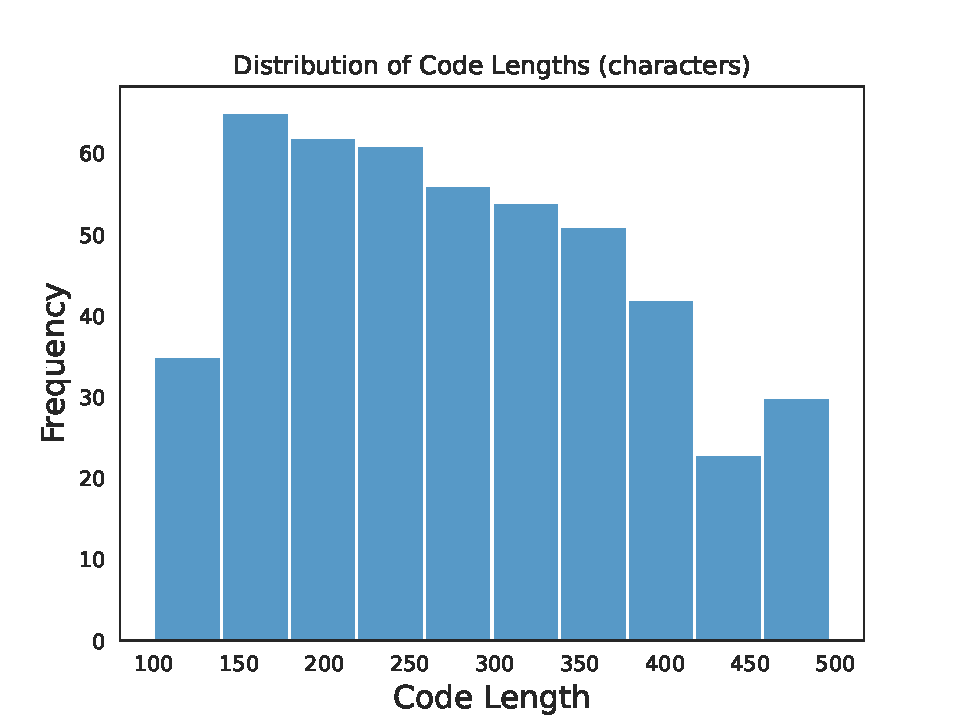
\includegraphics[width=0.48\textwidth]{figures/execution/code_lengths.pdf}
    \caption{Distribution of code lengths and number of execution steps}
    \label{fig:benchmark-filtering-size-selection}
\end{figure}

\rebuttal{
\subsection{Number of tests}
\label{app:subsec:num_tests}
We can sample large amounts of diverse inputs using our generator-based input sampling approach. 
However, the number of inputs produces a tradeoff in terms of the usability of the benchmark, slowing down the evaluation process. 
Hence, we threshold the number of sampled inputs to less than $25$ based on problem length, difficulty, and number of inputs.

We base this decision by estimating model performances when using different sets of inputs at random for testing in Figure~\ref{fig:teststudy}. Particularly, we vary the number of private tests between $0,\ 1,\ 5,\ 10,\ 20,\ 40,\ 60,\ 80,$ and $ 100$ and observe an exponentially decaying curve. We find the $\smallsim 20$ inputs provides a good threshold which balances evaluation time with evaluation rigor.


\begin{figure}
    \centering
    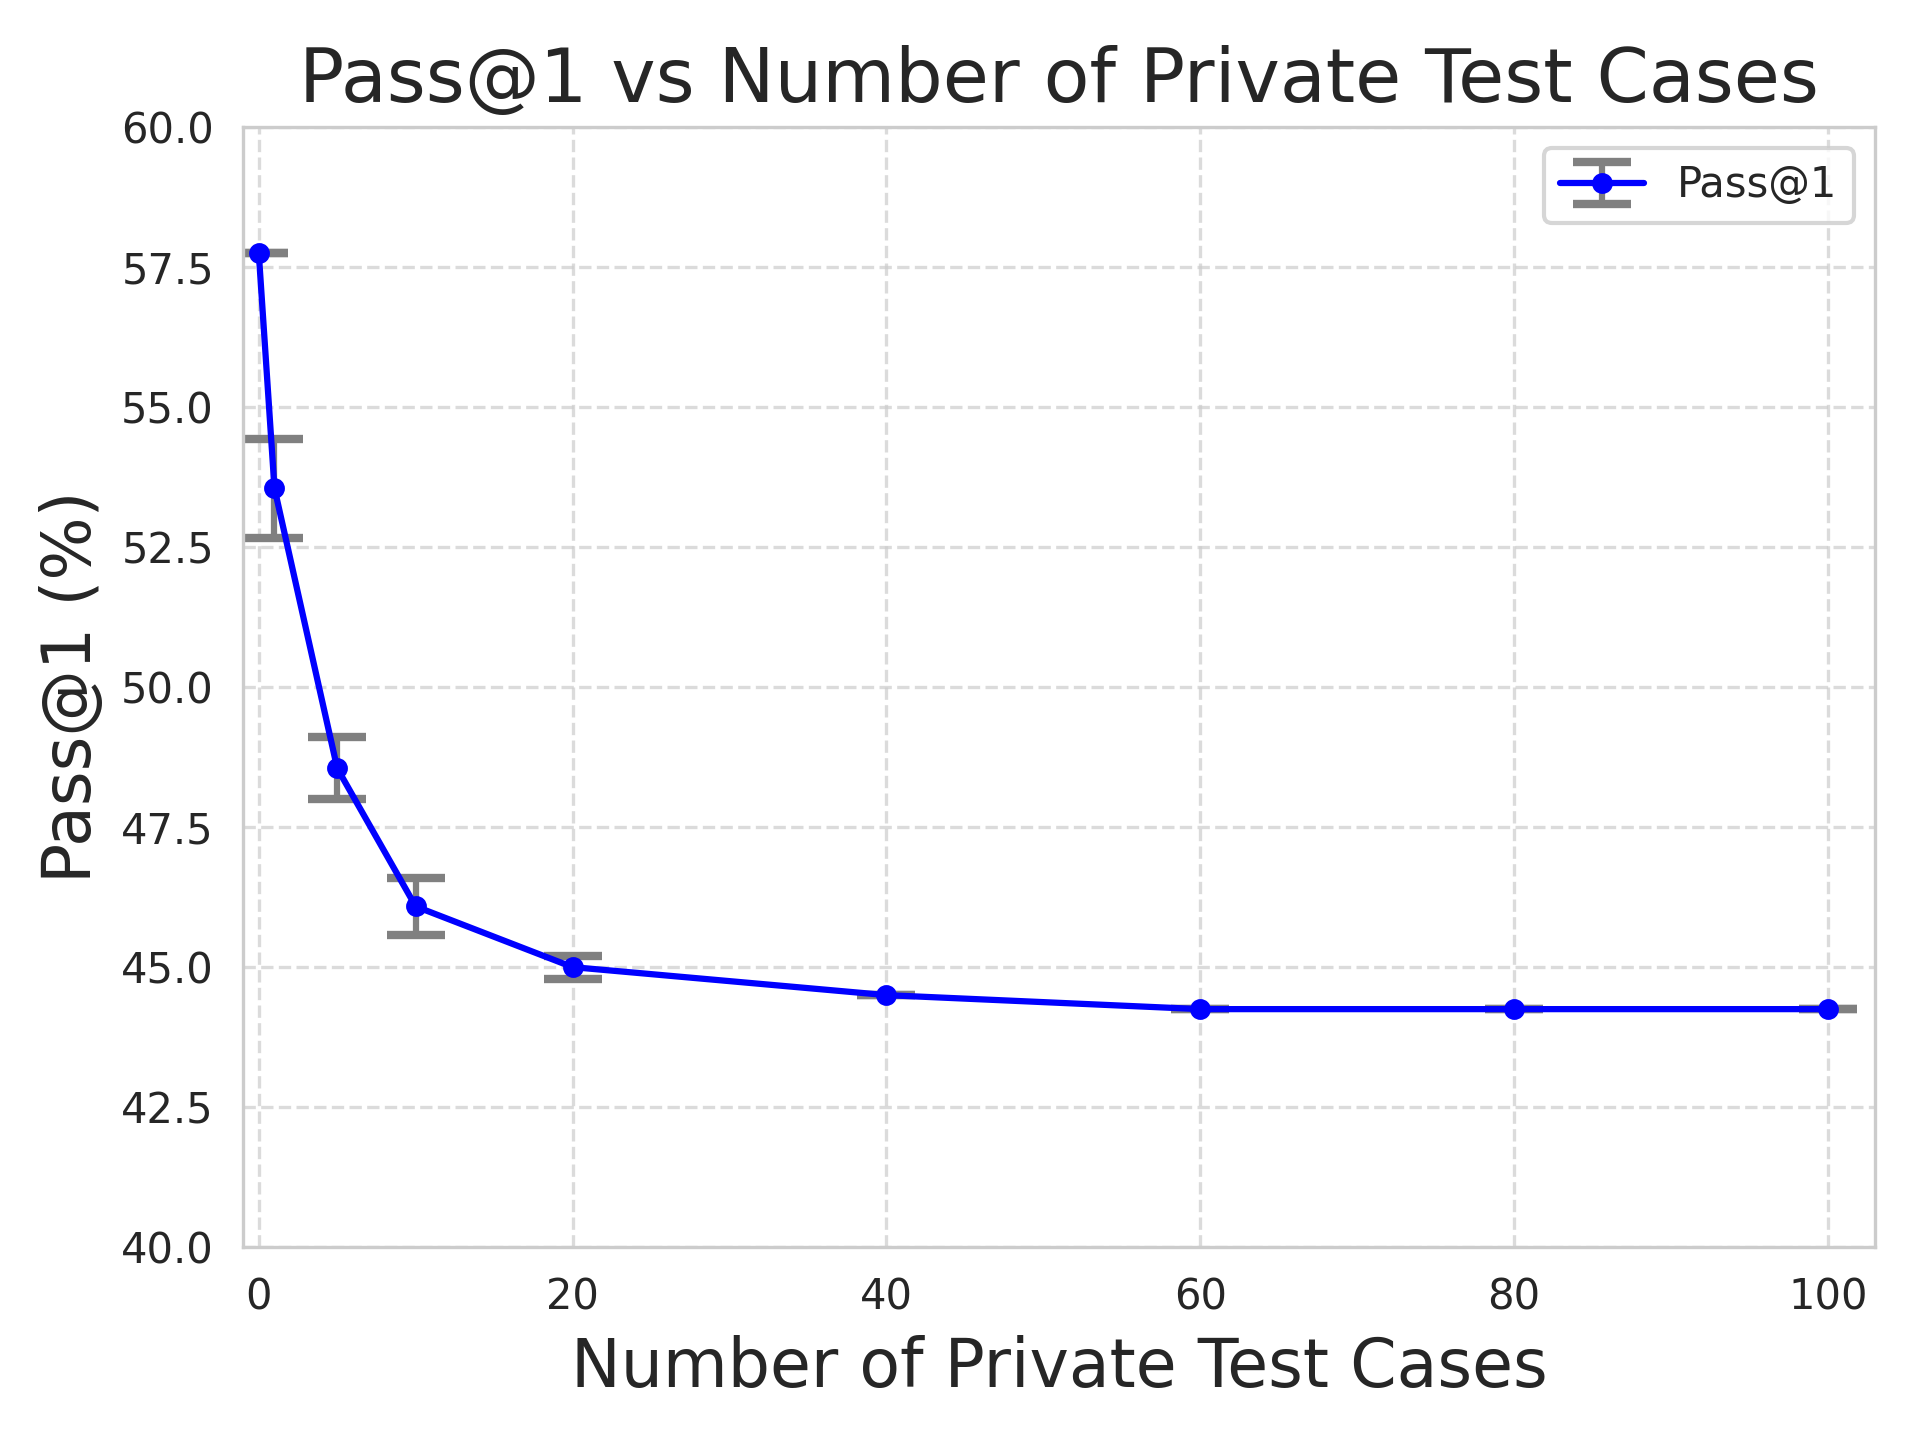
\includegraphics[width=0.7\linewidth]{figures/appendix/teststudy.png}
    \caption{Model performance with varying counts of private inputs used for evaluation. We find the \passmetric{1} tends to stabilize when sampling about $20$ inputs providing a good tradeoff in evaluation time and rigor.}
    \label{fig:teststudy}
\end{figure}

}